\documentclass{standalone}
\usepackage{pgfplots}

\begin{document}

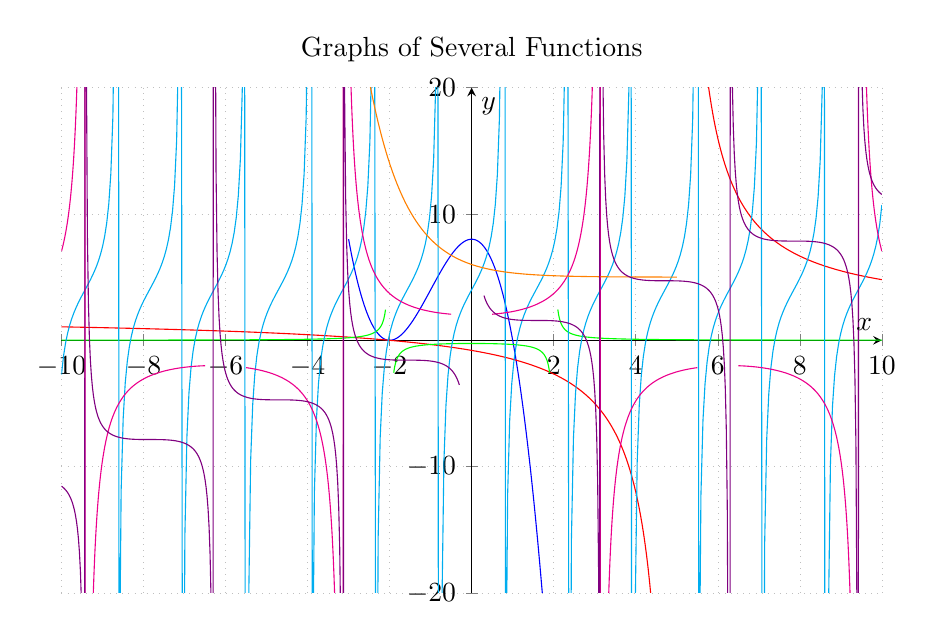
\begin{tikzpicture}
    \begin{axis}[
        xmin=-10,xmax=10,
        ymin=-20,ymax=20,
        xlabel={$x$},
        ylabel={$y$},
        axis lines=middle,
        grid=major,
        grid style={line width=.1pt, draw=gray!50, dotted},
        major grid style={line width=.2pt, draw=gray!50, dotted},
        width=12cm,
        height=8cm,
        title={Graphs of Several Functions}
    ]

    % Graph 1: y = -2x^3 - 6x^2 + 8
    \addplot[blue, domain=-3:2, samples=400] {-2*x^3 - 6*x^2 + 8};

    % Graph 2: y = (2x + 4) / (x - 5)
    \addplot[red, domain=-10:4.9, samples=400] {(2*x + 4)/(x - 5)};
    \addplot[red, domain=5.1:10, samples=400] {(2*x + 4)/(x - 5)};

    % Graph 3: y = 1 / (x^2 - 4)
    \addplot[green, domain=-10:-2.1, samples=400] {1/(x^2 - 4)};
    \addplot[green, domain=-1.9:1.9, samples=400] {1/(x^2 - 4)};
    \addplot[green, domain=2.1:10, samples=400] {1/(x^2 - 4)};

    % Graph 4: y = 3*tan(2x - pi) + 4
    \addplot[cyan, domain=-10:10, samples=400] {3*tan(deg(2*x - pi)) + 4};

    % Graph 5: y = 2*sec(0.5x)
    \addplot[magenta, domain=-10:-6.5, samples=400] {2/(cos(deg(0.5*x)))};
    \addplot[magenta, domain=-5.5:-0.5, samples=400] {2/(cos(deg(0.5*x)))};
    \addplot[magenta, domain=0.5:5.5, samples=400] {2/(cos(deg(0.5*x)))};
    \addplot[magenta, domain=6.5:10, samples=400] {2/(cos(deg(0.5*x)))};

    % Graph 6: y = 3^(-x) + 5
    \addplot[orange, domain=-5:5, samples=400] {3^(-x) + 5};

    % Graph 7: y = x + cot(x)
    \addplot[violet, domain=-10:-0.3, samples=400] {x + cot(deg(x))};
    \addplot[violet, domain=0.3:10, samples=400] {x + cot(deg(x))};

    \end{axis}
\end{tikzpicture}

\end{document}